\documentclass{article}
\usepackage[utf8]{inputenc}
\usepackage{graphicx}
\usepackage{amsmath}
\usepackage{amssymb}

\title{Mat4 Aflevering 4}
\author{Roar Nind Steffensen (s144107)}
\date{March 2016}

\begin{document}

\maketitle

\section*{Problem 4.17}

\begin{figure}[h!]
    \centering
    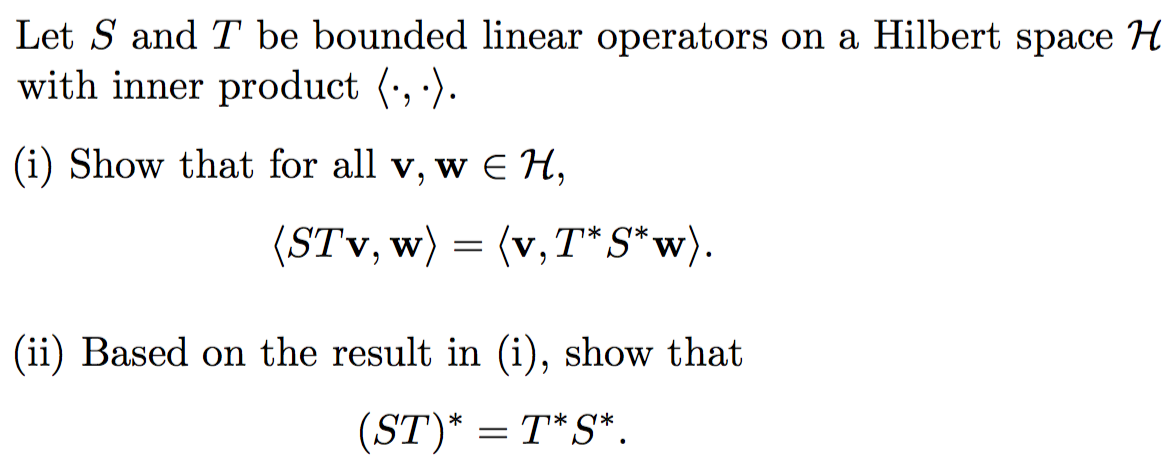
\includegraphics[width=\textwidth]{fig/prob417.png}
\end{figure}

\subsection*{Solution (i)}
First of, we assume that the adjoint operators $S^\ast$ and $T^\ast$ exist.\\
Then in order to know what to do with the two operators, we define $T\mathbf{v}$ as $\mathbf{v'}$, and $S^\ast\mathbf{w}$ as $\mathbf{w'}$ giving us a single operator of which we can find the adjoint operator.

\begin{gather*}
   \langle S T \mathbf{v},\mathbf{w}\rangle = \langle S \mathbf{v'},\mathbf{w}\rangle
\end{gather*}
\begin{gather*}
    \text{Using \textbf{Theorem 4.5.1} for adjoint operators and substituting} \\
   \langle S \mathbf{v'}, \mathbf{w} \rangle = \langle \mathbf{v'}, S^\ast \mathbf{w} \rangle = \langle T\mathbf{v}, \mathbf{w'} \rangle \\
    \langle T\mathbf{v}, \mathbf{w'} \rangle = \langle \mathbf{v}, T^\ast \mathbf{w'}= \langle \mathbf{v}, T^\ast S^\ast \mathbf{w} \rangle 
\end{gather*}

As we wanted.

\subsection*{Solution (ii)}

Using that if the operators were adjoint as a whole, we would get 

\begin{gather*}
    \langle S T \mathbf{v}, \mathbf{w} \rangle = \langle \mathbf{v}, (ST)^\ast \mathbf{w} \rangle
\end{gather*}

Meaning that 

\begin{gather*}
    \langle \mathbf{v}, T^\ast S^\ast \mathbf{w} \rangle = \langle \mathbf{v}, (ST)^\ast \mathbf{w} \rangle
\end{gather*}

\begin{gather*}
    \text{Using \textbf{lemma 4.4.2} } \\
    T^\ast S^\ast \mathbf{w}= (ST)^\ast \mathbf{w}
\end{gather*}

Which leaves us with the $(ST)^\ast$ and $T^\ast S^\ast$ being the same operator, as we wanted.

\section*{Problem 4.22}
\begin{figure}[h!]
    \centering
    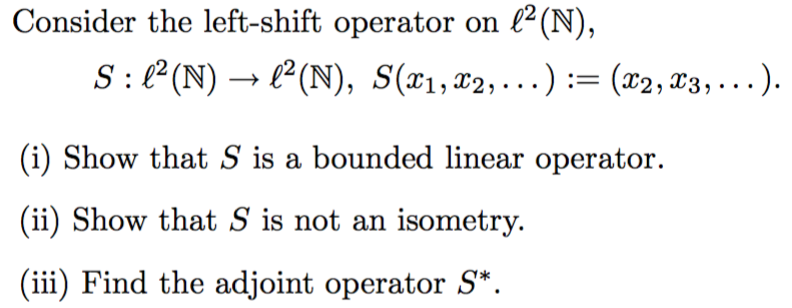
\includegraphics[width=10cm]{fig/prob422.png}
\end{figure}

\subsection*{Solution (i)}

First of we wish to show that $S$ is well defined.

\begin{gather*}
    || S(\{x_k\}) ||_2 = \left(\sum_{k=2}^\infty |x_k|^2 \right)^{1/2} \leq \left(\sum_{k=1}^\infty |x_k|^2 \right)^{1/2}
\end{gather*}

Which since $\{x_k\}$ must be in $l^2(\mathbb{N})$ this sum must be finite, leaving us with the conclusion that the operator is well defined.\\

Then we show that it is linear with using \textbf{equation 2.6} from \textbf{section 2.4}.

\begin{gather*}
    S( \alpha \{x_k\} + \beta \{y_k\}) = (\alpha x_2 + \beta y_2, \alpha x_3 + \beta y_3, ... )  \Rightarrow \\
     \alpha ( x_2, x,3,...) + \beta(y_2,y_3,...) = \alpha S(\{x_k\}) + \beta S(\{y_k\}) 
\end{gather*}

So the operator is linear, and to show that it is bounded, we start with the same argument as for the operator to be well defined together with \textbf{definition 2.4.1}.

\begin{gather*}
 || S(\{x_k\}) ||_2 = \left(\sum_{k=2}^\infty |x_k|^2 \right)^{1/2} \leq \left(\sum_{k=1}^\infty |x_k|^2 \right)^{1/2} = K ||\{x_k\}||_2 
 \end{gather*}
 
 With $K = 1$, which shows us that the operator is bounded.
 The operator is then a bounded linear operator. 
 
 \subsection*{Solution (ii)}
 
 Using \textbf{definition 2.4.5} stating that an operator $T$ is an isometry if $||T\mathbf{v}|| = ||v||$ for all $\mathbf{v} \in V_1$. We see that this is not the case, since $||S({x_k})||  \neq ||{x_k}||$ for $x_1 \neq 0$. And since this must hold for all sequences in our vector space, the operator is not an isometry. 

\subsection*{Solution (iii)}

By \textbf{equation 4.13} in \textbf{section 4.5}, using \textbf{theorem 4.5.1} and \textbf{theorem 4.2.1} we can find the adjoint operator $S^\ast$ as the sequence is given as

\begin{gather*}
    \langle S \{x_k\} , \{y_k\} \rangle = \sum_{k=1}^\infty x_{k+1}  \overline{y_k} =(x_2+\overline{y_1}+x_3+\overline{y_2}+...)
\end{gather*}

We wish to rewrite this so that we get a sequence from $x_1$ and forth

\begin{gather*}
    (x_2+\overline{y_1}+x_3+\overline{y_2}+...) = (x_1\cdot0+x_2+\overline{y_1}+x_3+\overline{y_2}+...)
\end{gather*}

Which in turn gives us the adjoint operator, which in this case is the right shift operator $S^\ast(\{y_k\})=(0,y_1,y_2,...)$.

\newpage
\section*{Problem 4.25 b)}

\begin{figure}[h!]
    \centering
    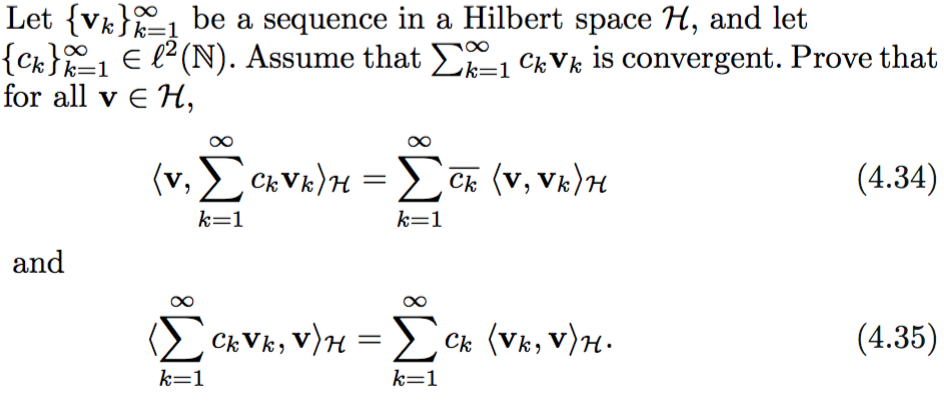
\includegraphics[width=12cm]{fig/prob425}
\end{figure}

\subsection*{Solution (4.35)}
Starting with the inner product in Hilbert space, using that the sum in "bra" of our inner product is a convergent sum, and that $\{\mathbf{v}_k \}$ is an infinite sequence in Hilbert space, giving us two infinite sums we can do the following.

\begin{gather*}
\text{Using \textbf{theorem 4.2.1}} \\
    \langle \sum_{k=1}^\infty c_k \mathbf{v}_k,\mathbf{v}\rangle = \sum_{n=1}^\infty \left( \sum_{k=1}^\infty c_k \mathbf{v}_k \right) \overline{\mathbf{v}_n} = \\
    \sum_{n=1}^\infty \left( \sum_{k=1}^\infty c_k \mathbf{v}_k \overline{\mathbf{v}_n} \right) = \sum_{k=1}^\infty \left( \sum_{n=1}^\infty c_k \mathbf{v}_k \overline{\mathbf{v}_n} \right) = \\
    \sum_{k=1}^\infty \left( c_k \sum_{n=1}^\infty \mathbf{v}_k \overline{\mathbf{v}_n} \right) = \sum_{k=1}^\infty c_k \langle \mathbf{v_k} , \mathbf{v} \rangle 
\end{gather*}

But it is unclear if the manipulation of sums always hold, since we have infinite linear combinations of vectors. Another approach would be to look at \textbf{definition 4.1.1 \textit{(i)}} which states that a linear combination of vectors in "bra" can be seen as a sum of scalars and inner products. 

\begin{gather*}
    \sum_{k=1}^n c_k \langle\mathbf{v}_k,\mathbf{v} \rangle
\end{gather*}

But as shown we only know that this is valid for finite sums. So in order to proof that this holds for an infinite, we must show that the sum converges to the infinite sum as $n\rightarrow \infty$. First of we look if the sum is a cauchy sequence

\begin{gather*}
    \left| \left|\sum_{k=1}^n c_k \langle\mathbf{v}_k,\mathbf{v} \rangle - \sum_{k=1}^l c_k \langle\mathbf{v}_k,\mathbf{v} \rangle \right| \right|_2 \leq 0 \: \: \text{whenever} \: \: n,l \geq N
\end{gather*}

Which can be show, since $\sum_{k=1}^\infty c_k \mathbf{v}_k$ is a convergent sum and $\{\mathbf{v}_k\}$ is in Hilbert space, which means that $\mathbf{v}_k$ must vanish as $k\rightarrow \infty$. The elements get smaller as $N\rightarrow \infty$, proofing that this in fact is a cauchy sequence. Using \textbf{lemma 3.1.3 } this cauchy sequence converges, meaning that

\begin{gather*}
    \langle \sum_{k=1}^\infty c_k \mathbf{v}_k,\mathbf{v}\rangle = \sum_{k=1}^\infty c_k \langle\mathbf{v}_k,\mathbf{v} \rangle
\end{gather*}

As we wanted.

\end{document}
